% Robert Adams CS 475

\documentclass[letterpaper,10pt]{article} %twocolumn titlepage 
\usepackage{graphicx}
\usepackage{amssymb}
\usepackage{amsmath}
\usepackage{amsthm}

\usepackage{alltt}
\usepackage{float}
\usepackage{color}
\usepackage{url}

\usepackage{balance}
\usepackage[TABBOTCAP, tight]{subfigure}
\usepackage{enumitem}
\usepackage{pstricks, pst-node}


\usepackage{geometry}
\geometry{margin=0.8in, textheight=8.5in} %textwidth=6in

%random comment

\newcommand{\cred}[1]{{\color{red}#1}}
\newcommand{\cblue}[1]{{\color{blue}#1}}

\usepackage{hyperref}

\def\name{Robert Adams}
%% The following metadata will show up in the PDF properties
\hypersetup{
	colorlinks = true,
	urlcolor = black,
	pdfauthor = {\name},
	pdfkeywords = {cs745},
	pdftitle = 	{CS 475 Project 9: OpenCL / OpenGL Particle System},
pdfsubject = {CS 475 Project 9},
	pdfpagemode = UseNone,
}


\begin{document}
\title{CS 475 Project 9: OpenCL / OpenGL Particle System}
\author{Robert Adams}
\maketitle



\section{Commentary}

\indent First thing to note: GPU performance absolutely destroys SIMD performance,
iny my case by a factor of over 50x. 
\\
Also of note is that modifying local work size does not affect the 
performance. I was not able to see a difference on either my home 
system (specs below), or the CGEL lab. This may be because the video
cards of both are rather out of date.  For a new, or properly setup
machine we should see performance increase as the local size increases,
since more processing power has been assigned to the task.

\subsection{System Specs}

\begin{itemize}
\item Processor: Intel(R) Xeon(R) CPU   W3550  @ 3.07GHz, 3060 Mhz, 4 Core(s), 4 Logical Processor(s)
\item RAM: 8.00 GB
\item OS Name \& Version: Microsoft Windows 7 Enterprise 6.1.7601 Service Pack 1 Build 7601
\item Video Card: NVIDIA GeForce GTX 480 
\item Adapter RAM: 1.50 GB (1,610,285,056 bytes) 
\item Driver Version: 8.17.13.132
\end{itemize}


\pagebreak

\begin{figure} [ht]
	\centering
	% GNUPLOT: LaTeX picture with Postscript
\begingroup
  \makeatletter
  \providecommand\color[2][]{%
    \GenericError{(gnuplot) \space\space\space\@spaces}{%
      Package color not loaded in conjunction with
      terminal option `colourtext'%
    }{See the gnuplot documentation for explanation.%
    }{Either use 'blacktext' in gnuplot or load the package
      color.sty in LaTeX.}%
    \renewcommand\color[2][]{}%
  }%
  \providecommand\includegraphics[2][]{%
    \GenericError{(gnuplot) \space\space\space\@spaces}{%
      Package graphicx or graphics not loaded%
    }{See the gnuplot documentation for explanation.%
    }{The gnuplot epslatex terminal needs graphicx.sty or graphics.sty.}%
    \renewcommand\includegraphics[2][]{}%
  }%
  \providecommand\rotatebox[2]{#2}%
  \@ifundefined{ifGPcolor}{%
    \newif\ifGPcolor
    \GPcolorfalse
  }{}%
  \@ifundefined{ifGPblacktext}{%
    \newif\ifGPblacktext
    \GPblacktexttrue
  }{}%
  % define a \g@addto@macro without @ in the name:
  \let\gplgaddtomacro\g@addto@macro
  % define empty templates for all commands taking text:
  \gdef\gplbacktext{}%
  \gdef\gplfronttext{}%
  \makeatother
  \ifGPblacktext
    % no textcolor at all
    \def\colorrgb#1{}%
    \def\colorgray#1{}%
  \else
    % gray or color?
    \ifGPcolor
      \def\colorrgb#1{\color[rgb]{#1}}%
      \def\colorgray#1{\color[gray]{#1}}%
      \expandafter\def\csname LTw\endcsname{\color{white}}%
      \expandafter\def\csname LTb\endcsname{\color{black}}%
      \expandafter\def\csname LTa\endcsname{\color{black}}%
      \expandafter\def\csname LT0\endcsname{\color[rgb]{1,0,0}}%
      \expandafter\def\csname LT1\endcsname{\color[rgb]{0,1,0}}%
      \expandafter\def\csname LT2\endcsname{\color[rgb]{0,0,1}}%
      \expandafter\def\csname LT3\endcsname{\color[rgb]{1,0,1}}%
      \expandafter\def\csname LT4\endcsname{\color[rgb]{0,1,1}}%
      \expandafter\def\csname LT5\endcsname{\color[rgb]{1,1,0}}%
      \expandafter\def\csname LT6\endcsname{\color[rgb]{0,0,0}}%
      \expandafter\def\csname LT7\endcsname{\color[rgb]{1,0.3,0}}%
      \expandafter\def\csname LT8\endcsname{\color[rgb]{0.5,0.5,0.5}}%
    \else
      % gray
      \def\colorrgb#1{\color{black}}%
      \def\colorgray#1{\color[gray]{#1}}%
      \expandafter\def\csname LTw\endcsname{\color{white}}%
      \expandafter\def\csname LTb\endcsname{\color{black}}%
      \expandafter\def\csname LTa\endcsname{\color{black}}%
      \expandafter\def\csname LT0\endcsname{\color{black}}%
      \expandafter\def\csname LT1\endcsname{\color{black}}%
      \expandafter\def\csname LT2\endcsname{\color{black}}%
      \expandafter\def\csname LT3\endcsname{\color{black}}%
      \expandafter\def\csname LT4\endcsname{\color{black}}%
      \expandafter\def\csname LT5\endcsname{\color{black}}%
      \expandafter\def\csname LT6\endcsname{\color{black}}%
      \expandafter\def\csname LT7\endcsname{\color{black}}%
      \expandafter\def\csname LT8\endcsname{\color{black}}%
    \fi
  \fi
  \setlength{\unitlength}{0.0500bp}%
  \begin{picture}(8640.00,5040.00)%
    \gplgaddtomacro\gplbacktext{%
      \csname LTb\endcsname%
      \put(1342,704){\makebox(0,0)[r]{\strut{} 1.85}}%
      \put(1342,1156){\makebox(0,0)[r]{\strut{} 1.9}}%
      \put(1342,1609){\makebox(0,0)[r]{\strut{} 1.95}}%
      \put(1342,2061){\makebox(0,0)[r]{\strut{} 2}}%
      \put(1342,2514){\makebox(0,0)[r]{\strut{} 2.05}}%
      \put(1342,2966){\makebox(0,0)[r]{\strut{} 2.1}}%
      \put(1342,3419){\makebox(0,0)[r]{\strut{} 2.15}}%
      \put(1342,3871){\makebox(0,0)[r]{\strut{} 2.2}}%
      \put(1342,4324){\makebox(0,0)[r]{\strut{} 2.25}}%
      \put(1342,4776){\makebox(0,0)[r]{\strut{} 2.3}}%
      \put(1474,484){\makebox(0,0){\strut{} 1e+06}}%
      \put(2158,484){\makebox(0,0){\strut{} 2e+06}}%
      \put(2841,484){\makebox(0,0){\strut{} 3e+06}}%
      \put(3525,484){\makebox(0,0){\strut{} 4e+06}}%
      \put(4208,484){\makebox(0,0){\strut{} 5e+06}}%
      \put(4892,484){\makebox(0,0){\strut{} 6e+06}}%
      \put(5576,484){\makebox(0,0){\strut{} 7e+06}}%
      \put(6259,484){\makebox(0,0){\strut{} 8e+06}}%
      \put(6943,484){\makebox(0,0){\strut{} 9e+06}}%
      \put(7626,484){\makebox(0,0){\strut{} 1e+07}}%
      \put(8310,484){\makebox(0,0){\strut{} 1.1e+07}}%
      \put(440,2740){\rotatebox{90}{\makebox(0,0){\strut{}GigaParticles/sec}}}%
      \put(4892,154){\makebox(0,0){\strut{}particles}}%
    }%
    \gplgaddtomacro\gplfronttext{%
    }%
    \gplbacktext
    \put(0,0){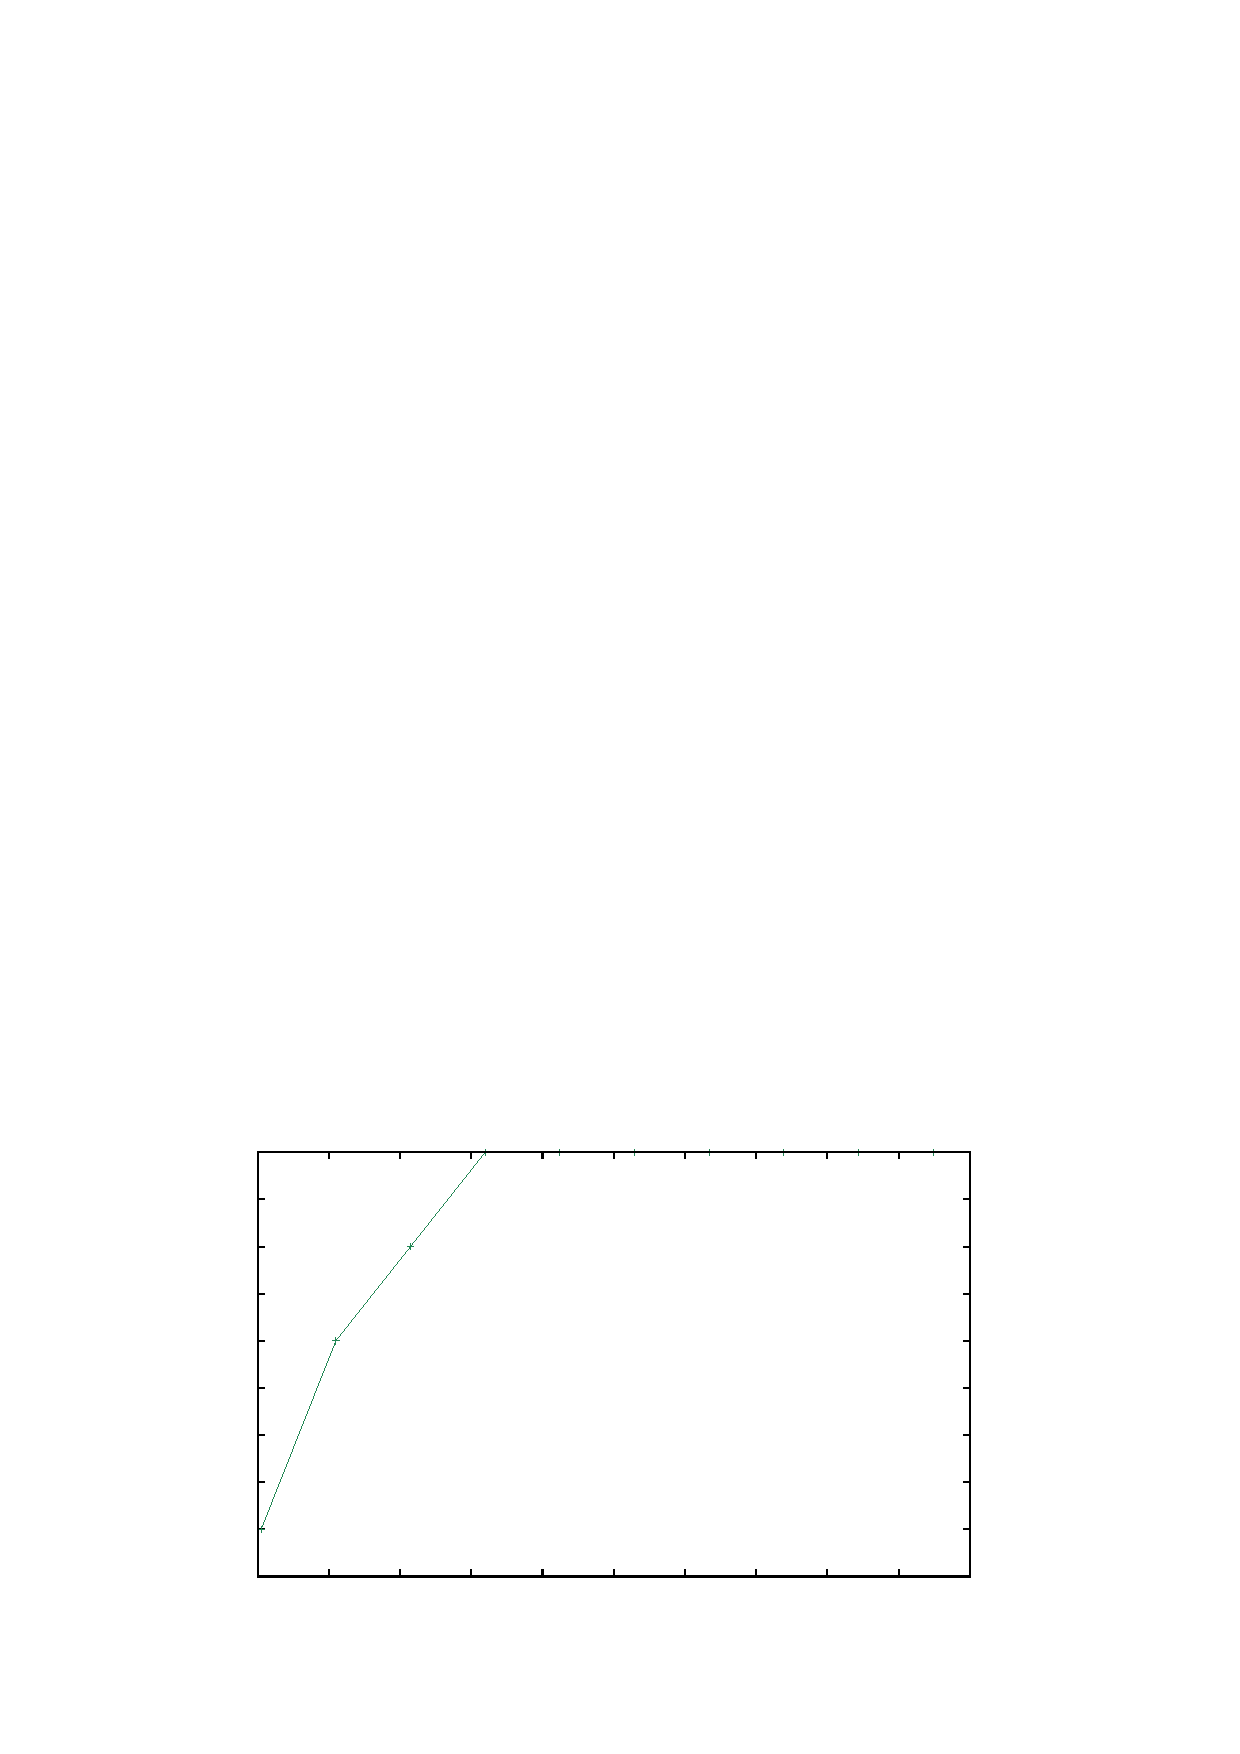
\includegraphics{graph}}%
    \gplfronttext
  \end{picture}%
\endgroup

	%\caption{Speed of height calculations performed on a subdivided surface} 
	\label{runtimes}
\end{figure}

\begin{table}  [ht]
    \centering
        \begin{tabular}{llllll}
        \verb|#| of particles & GigaParticles/sec \\ \hline 
                      1048576 & 1.9\\ 
                      2097152 & 2.1\\ 
                      3145728 & 2.2\\ 
                      4194304 & 2.3\\ 
                      5242880 & 2.3\\ 
                      6291456 & 2.3\\ 
                      7340032 & 2.3\\ 
                      8388608 & 2.3\\ 
                      9437184 & 2.3\\ 
                     10485760 & 2.3
            \end{tabular}
    \end{table}

    \end{document}
